\documentclass[journal]{IEEEtran}
\usepackage{graphicx}
\usepackage[utf8]{inputenc}
\ifCLASSINFOpdf
\else
\fi
\hyphenation{op-tical net-works semi-conduc-tor}
\begin{document}
\title{Generador de Kakuros}
\author{Eduard~Torres~Chaves,~\IEEEmembership{}
        y~Juan~José~Solano~Quesada,~\IEEEmembership{}
\thanks{E. Torres Chaves estudiante de Ingeniería en computación, Instituto Tecnológico de Costa Rica}% <-this % stops a space
\thanks{J.J. Solano estudiante de Ingeniería en computación, Instituto Tecnológico de Costa Rica}% <-this % stops a space
\thanks{}}
\maketitle
\begin{abstract}
The project is about solving Kakuro's puzzles using backtracking, threads and forks. First we start discussing and analyzing the different sections of the backtracking and the backtracking itself. Then we explore the possibility to implement threads and then after implementing them we compare the results to see if the thread implementation is better than the normal one using as reference two experiments. Then we discuss the posibility of doing it with forks.

\end{abstract}
\begin{IEEEkeywords}
Backtracking, thread, poda.
\end{IEEEkeywords}
\IEEEpeerreviewmaketitle

\section{Introducción}
Un kakuro es un juego matemático que consiste en un conjunto de casillas blancas y negras, en las cuales se deben rellenar las casillas blancas en el tablero con números del 1 al 9 tal que las suma de los valores en las casilla sea igual a la clave que se encuentra a la izquierda para las filas y por encima de las columnas.\\
Entre sus reglas se distinguen que no se puede repetir el valor de una casilla en la misma fila y columna hasta que haya un espacio negro y, por ende, la cantidad máxima de celdas consecutivas es 9.\\
Los problemas matemáticos que representan estos enigmas pueden resolverse utilizando tecnicas de matriz matemática y backtracking.

\begin{figure}[h] 
        \centering 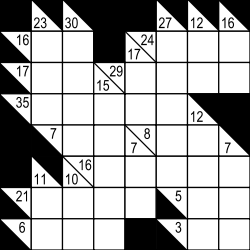
\includegraphics[width=.35\columnwidth]{kakuro_blank.png}
        \caption{
                \label{fig:samplesetup}
                Ejemplo de kakuro sin resolver
        }
\end{figure}

\begin{figure}[h] 
        \centering 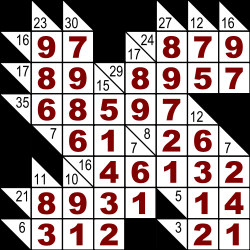
\includegraphics[width=.35\columnwidth]{kakuro_solved.png}
        \caption{
                \label{fig:samplesetup}
                Ejemplo de kakuro resuelto
        }
\end{figure}

\section{Análisis}
\subsection{Generar un tablero}


\end{document}